\section{Proposed Research}
\label{sec:proposed-work}
%The proposed research develops fast,
%high-order-accurate, parallel numerical algorithms for large-scale
%simulations of the collective hydrodynamics of amphiphilic particles in a viscous solvent.
%%
We have demonstrated that our hydrophobic attraction with repulsion potential (HARP) approach efficiently simulates
self-assembly of amphiphilic particles into two-dimensional micelles, bilayer membranes, and vesicles \cite{Fu2018_SIAM}, and
recreates the tank-treading phenomenon in external shear flows
\cite{Fu20}.
%\todo[inline]{!!let's put a proceedings here so we have something to cite!!}.
%
While the results show great promise in the field of collective body hydrodynamics,
several outstanding issues need to be addressed. These include a thorough 
analysis of elastic properties of our coarse-grained bilayers, and 
efficiently simulating three-dimensional collective hydrodynamics of amphiphilic particles.
Finally, we must mathematically characterize the variational behavior of HARP under appropriate homogenized limits.

\subsection{Specific Aim 1: Material properties of self-assembly of amphiphiles}
\label{subsec:specific_aim_1}

%\begin{figure}
%\begin{center}
%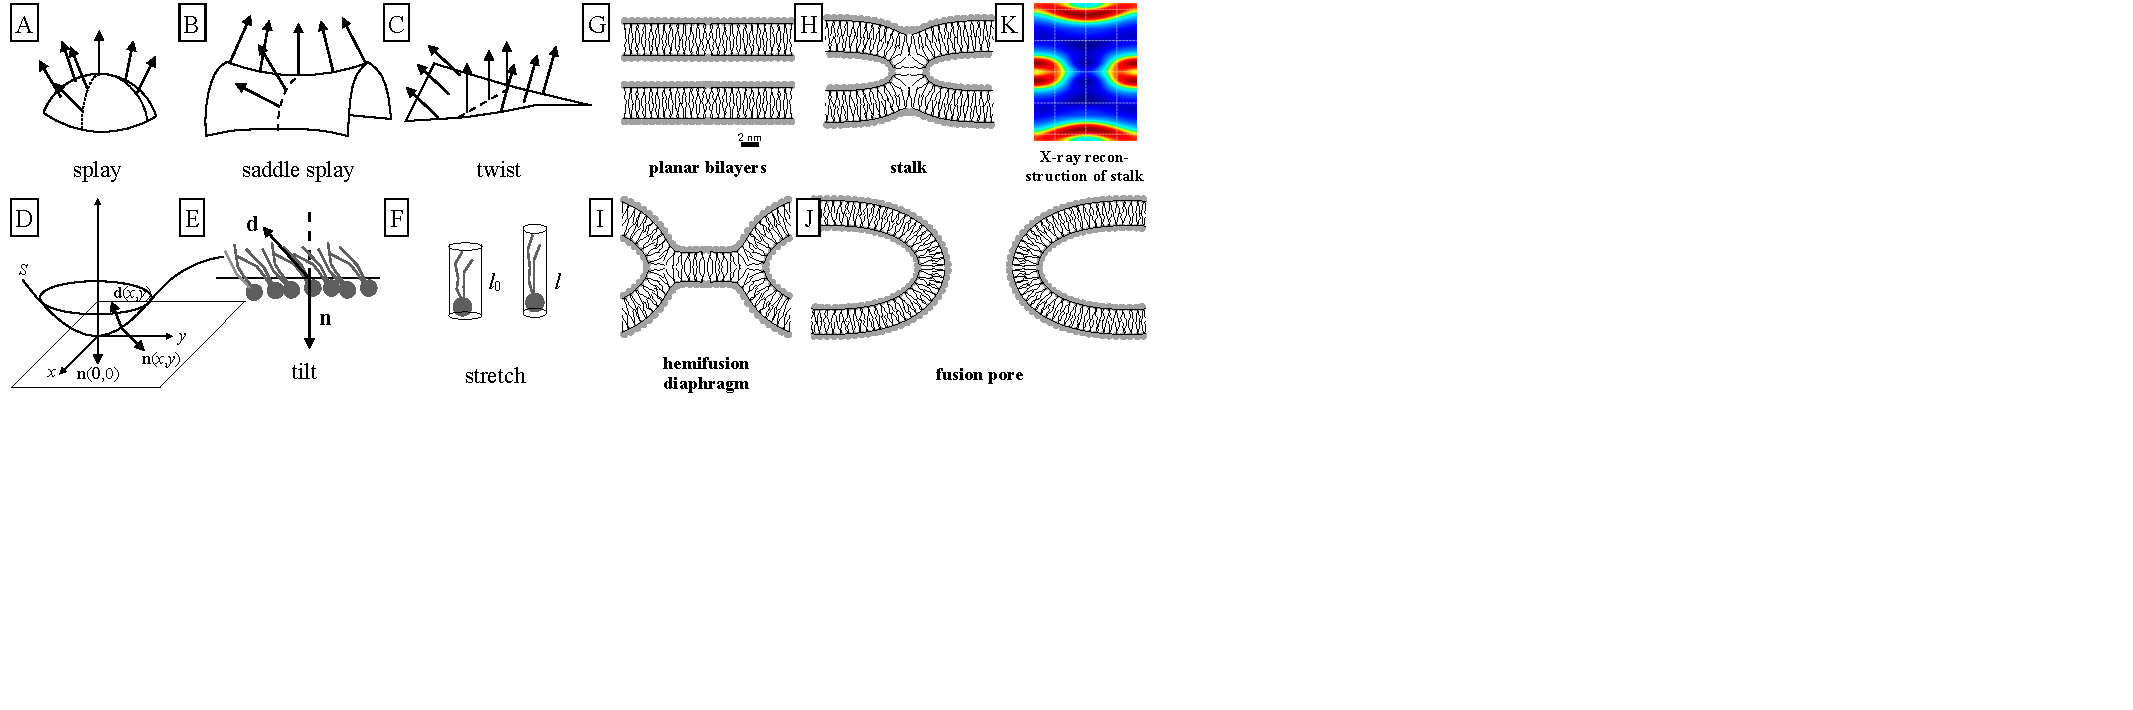
\includegraphics[width=0.9\textwidth]{figures/SA1_fig1.pdf}
%\end{center}
%\caption{\footnotesize (A--C) The splay ($\Div \mathbf{d}$), 
%saddle splay ($\det \mathsf{D}$) and twist ($\Curl \mathbf{d}$) elastic distortions of 
%a monolayer. (D) The monolayer neutral surface $\Sigma$,  
%director $\mathbf{d}$ and unit normal $\mathbf{n}$ in local coordinates.
%(E--F) Lipids are able to tilt from  the surface normal, and stretch.
%(H--J) Intermediates of membrane fusion and (K) experimental image of a stalk \cite{Aeffner2012}. }
%\label{fig:distortions}
%\end{figure}
The goal of Specific Aim 1 is characterize the material properties of many-body, self-assembled amphiphiles.
For amphiphiles assembled into bilayers, these properties are described by membrane continuum mechanics.
Our goal is to be able to map the parameters of the particle-based model onto the elastic moduli from continuum theory.
Results from this goal will facilitate simulators to use the hydrophobic attraction force calculations
to model bilayers with specific composition. These calculations have provably less computational complexity than
those of molecular dynamics simulations and possess the molecular granularity lacking from continuum models.

The modern theory of membrane continuum mechanics 
was pioneered by Hamm and Kozlov (HK) \cite{Hamm2000}.
The theory is widely used to describe biological phenomona 
fission \cite{FrEsAkSh15, Maetal15, PhysRevE.79.031926},
fusion \cite{ChKo08, KoKo2002,Kuzmin7235,Aeffner2012},
poration \cite{Gaetal20}, phase boundaries and interaction with inclusions
\cite{SeLeMaEg17,Saetal20, Pietal20}, which require resolution of the internal structure of the membrane.  
Using the HK  model as a base,
PI Ryham and collaborators calculated, for the first time in continuum theory, a least energy path for transitions between planar bilayers, a membrane stalk,
hemifusion diaphragm and the fusion pore \cite{RyWaCo13,RyKlYaCo16},
and the energies calculated by these continuum studies (Figure \ref{fig:barriers}A),
are in agreement with barrier heights derived by molecular dynamics and experimental studies \cite{FrRoPi17}.  

Recently, there has been a revival in interest in the HK theory. The quadratic assumption
for the elasticity energy density has caused researchers to question the applicability of \eqref{ansatz3} for large curvatures \cite{PhysRevLett.117.188102, ARGUDO20161619}. 
The article \cite{C9SM02079A} counters that energies derived from molecular dynamics and elasticity agree, even when curvatures are large.
This proposal will bring mathematical analysis to some of the assumptions 
that went into the HK theory. 

The HK framework assumes a three-dimensional, internal structure for lipid monolayers.
The internal structure consists of straight fibers that represent elongated hydrocarbon chains, and these fibers
tilt and stretch with respect to the dividing surface--the surface formed lying between the hydrocarbon chains and polar heads of lipids.
Accordingly, the deformation takes the form 
\begin{equation}
  \label{LMdeformation}
x(X_1, X_2, X_3) = x_0(X_1, X_2) + \zeta(x_0(X_1, X_2), X_3) n(x_0(X_1, X_2))
\end{equation}
where $(X_1,X_2,X_3)$ are points in a reference volume.
The map $x_0$ parametrizes the dividing surface $\Sigma$, and the unit vector field $n$ parametrizes the
direction of the lipid tails in the deformed state \cite{doi:10.1021/jp075641w,KLAUDA20083074}.
The parameter $X_3$ and the function $\zeta$ parametrizes the distance along the hydrocarbon chain in the reference state
and the deformed state, respectively, and so $0 \leq X_3 \leq \delta$ where $\delta = $ 2.5 nm is a realistic monolayer thickness. 

The elastic theory assumes an energy density that is quadratic in the Green-Lagrange strain tensor for $x$. 
The chains stretch and compress to satisfy incompressibility.
Symmetries with respect to mirror reflection and in-plane rotation, the internal structure assumptions and incompressibility
lead to an elastic surface energy over the dividing surface $\Sigma$. 
This energy decomposes into four, fundamental and independent deformations:
splay ($\Div n$), twist ($\Curl n$), saddle splay ($\det \nabla n$) and tilt $T$:
\begin{equation}
\label{ansatz3}
\begin{aligned}
\int_{\Sigma} 
  \tfrac{1}{2}\KB\left[ \left( \Div n + k_0\right)^2 - k_0^2\right] 
+ \tfrac{1}{2}\KT (\Curl n)^2 + \KG  \det \nabla n + \tfrac{1}{2}\KTH |T|^2 \,dA.
\end{aligned}
\end{equation}
Here $\Div n$, $\Curl n$ and $\nabla n$ refer to the surface divergence, surface curl and surface gradient operators
respectively (Figure \ref{fig:distortions}A--C).
The deformations come with elastic coefficients: the bending modulus $\KB$, twist modulus $\KT$ 
and saddle-splay modulus $\KG$ and tilt modulus $\KTH$
HK define the tilt vector $T = n/(N\cdot n) - N$ where $N$ is the unit surface normal.

The parameter $k_0$ is the  spontaneous curvature and it determines the preferred lipid splay \cite{RoLi15,Kozlov2007}. 
As an illustration, the lipid DSPC has $k_0 = -0.1$ nm$^{-1}$ 
%as a result of  %having a relatively long acyl chain. 
and these lipids would line the  inner monolayer of a 
spherical liposome, because the addition of a positive splay $\Div \mathbf{d}$  in \eqref{ansatz3}
to the negative spontaneous curvature $k_0$ leads to lower energy \cite{Kamal22245, C3SM51829A, RoLi15,FriedSeguin15}.
The subtraction of $k_0^2$ makes the energy distortion free
\cite{Helfrich73,PhysRevLett.113.248102,Hamm2000}.

An interesting and challenging feature of \eqref{ansatz3} is that the
elastic energy couples director gradients to surface geometry through
the tilt vector field.  In biological contexts, bilayer energy is the
sum monolayer energies, and tilt appears at lipid domain boundaries, the
edge of nanopores and at the boundary of membrane inclusions
\cite{PhysRevE.102.042406}.  Under spatial scales much larger than the
membrane thickness, membrane energy is well-characterized by the
Canham-Helfrich energy used throughout the fluid-structure literature
\cite{QiangDu09, Lowengrub07,KimLai2010_JCP, Hu, HuLaiSeolEtAl2016_JCP,
qua-bir2014, qua-vee-you2019}. \todo[inline]{YNY: place your recent
works here} The Canham-Helfrich energy is actually a special case of
\eqref{ansatz3} obtained by setting $n =  \pm N$ (the $\pm$ depending on
orientation) and collapsing both monolayers onto the membrane midplane.
There, splay $\Div n$ equal to twice the mean curvature, saddle splay
$\det \nabla n$ equal to the Gauss curvature, and both twist and tilt
are equal to zero. 



%\begin{figure}
%\begin{center}
%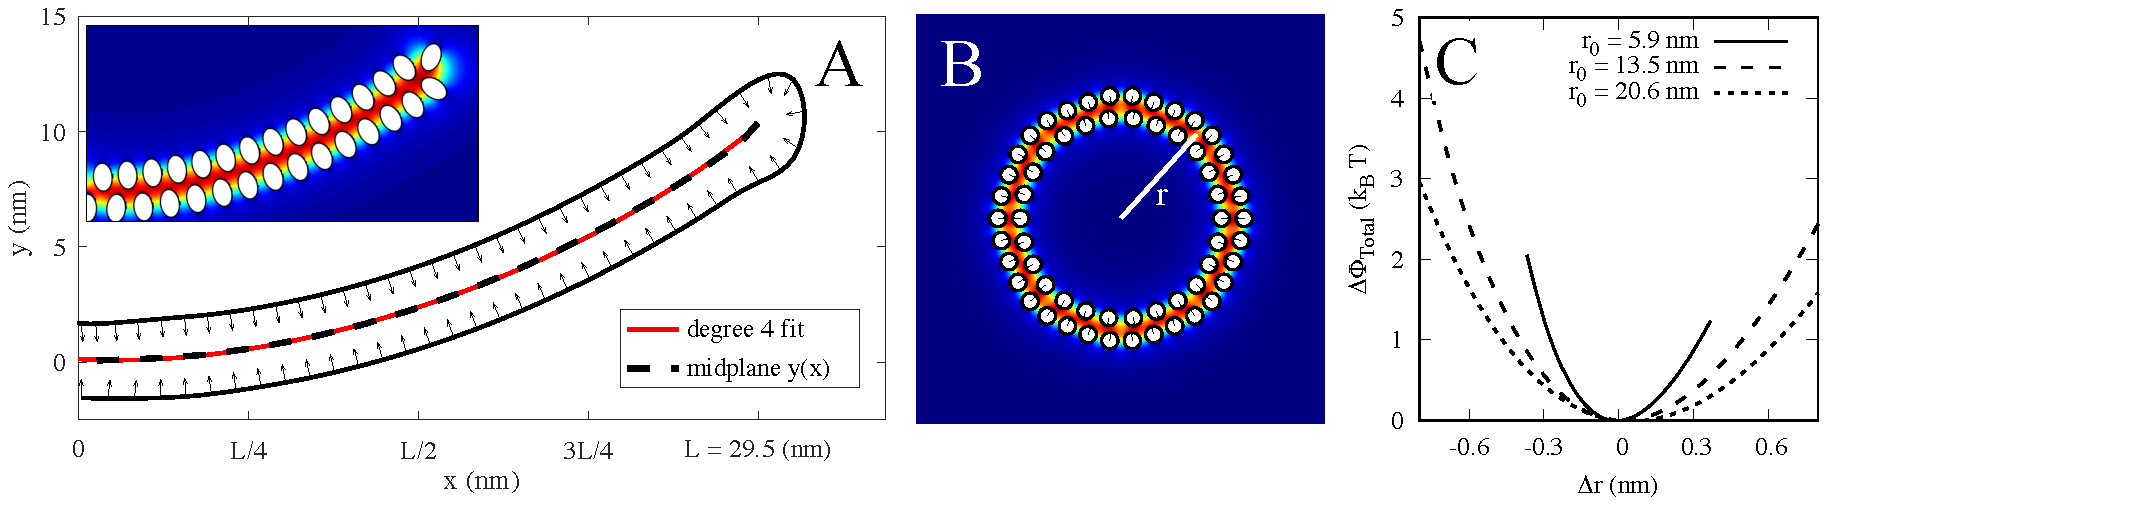
\includegraphics[width=\textwidth]{figures/SA1_fig2.pdf}
%\end{center}\vspace{-1.em}
%\caption{\footnotesize (A) A partially clamped bilayer with mid-plane (dashed curve) under uniform load.
%The quartic fit comes from continuum theory. 
%(B) A circular vesicle at equilibrium. (C) The area modulus derives
%from convexity in energy as a function of radius. 
%\label{fig:bend}}
%\end{figure}


% Proposers should address what they want to do,
% why they want to do it,
% how they plan to do it,
% how they will know if they succeed,
% and what benefits could accrue if the project is successful.
%\begin{center}
%Preliminary results
%\end{center}
\subsubsection{Preliminary results}
Our preliminary tested for elastic properties by subjecting bilayers to external loads \cite{Fu2018_SIAM}.
We used realistic values for the phospholipid length $a$ \cite{Boal},
screening length $\rho = 2.5$ nm \cite{Eriksson1989,Lin2005,Parsegian,Israelachvili80,TerziDeserno17}
and interfacial tension $\gamma=4.1$ pN nm$^{-1}$ \cite{GarciaSaez, KUZMIN2005, Petelska2012, Jackson}
model parameters.
The repulsion strength, repulsion length scale, particle shape (e.g. disks, ellipses), 
particle diameter and the hydrophobic boundary condition \eqref{SL}
are additional parameters defining the coarse-grained representation. 

To derive a bending modulus, we first considered a planar bilayer subject to a uniform vertical load on the particle centers (Figure \ref{fig:bend}). 
Using a clamped condition at one end, the restoring force in the free part of the bilayer opposes the load.
For small deformations, it is possible to solve the bilayer loading in closed form, and 
this analytical solution (red curve) basically overlaps the midplane of the particle based solution (Figure \ref{fig:bend}A).
We thereby derived a bending modulus $\KB$ in the range 8.51 -- 13.54 \kBT. Throughout the proposal, \kBT\; = 4.11$\times 10^{-21}$ J.
Experimental measurements have accurately determined the bending modulus for several lipid types, with 
typical values lying around 10 \kBT\; \cite{Naetal15,VeBrPa15,NAGLE2000159,PhysRevLett.113.248102}.

We also considered the stretching and tilt deformations \cite{Fu2018_SIAM}. 
Stretching occurs whenever there is an excess monolayer area,
and it is energetically costly since it exposes hydrocarbon tails to water.
To measure an area modulus, we stretched a circular vesicle, modeling the cross-section 
of a bilayer tube (Figure \ref{fig:bend}B \& C).
This procedure gave a monolayer area modulus 
34 $\pm$ 2 \kBT \;nm$^{-2}$. Manipulation experiments give a monolayer area modulus in the range 
30 -- 40 \kBT\; nm$^{-2}$ \cite{Nagle17, Nagle17-2}. 

Finally, we considered the tilt deformation by applying a fixed tilt angle boundary condition. 
This boundary condition produces a tilt field that decays with the length scale $l = \sqrt{\KB/\KTH}$ 
Fitting to this field, our particle based simulation gave $\lambda = 1.2$ nm, which matches
the value $\KTH \approx 10$ \kBT \; nm$^{-2}$ reported in the literature \cite{KUZMIN2005, KoNa15}.

Our preliminary work is encouraging because in all cases, the bending, stretch, and tilt elastic moduli for the collection of amphiphiles
were in excellent agreement with the experimental values. This fact is especially remarkable 
since we assigned the main model parameters $\rho$ and $\gamma$ reasonable physical values, rather than using them as tuning parameter. 
Nevertheless, the characterization of material properties is incomplete. For one, the preliminary simulations involved relatively low particle numbers (20 to 30), and so we still need to
perform convergence studies with large particle-number systems to arrive at conclusive results. Secondly, we have yet to establish a functional
relationship between the model parameters and elastic moduli. Finally, to have relevance in physics and biology
we must incorporate the remaining twist and saddle splay deformations.
The following simulation outline shows how will achieve aims. 


%\begin{wrapfigure}[13]{l}{0.5\textwidth}
%\centerline{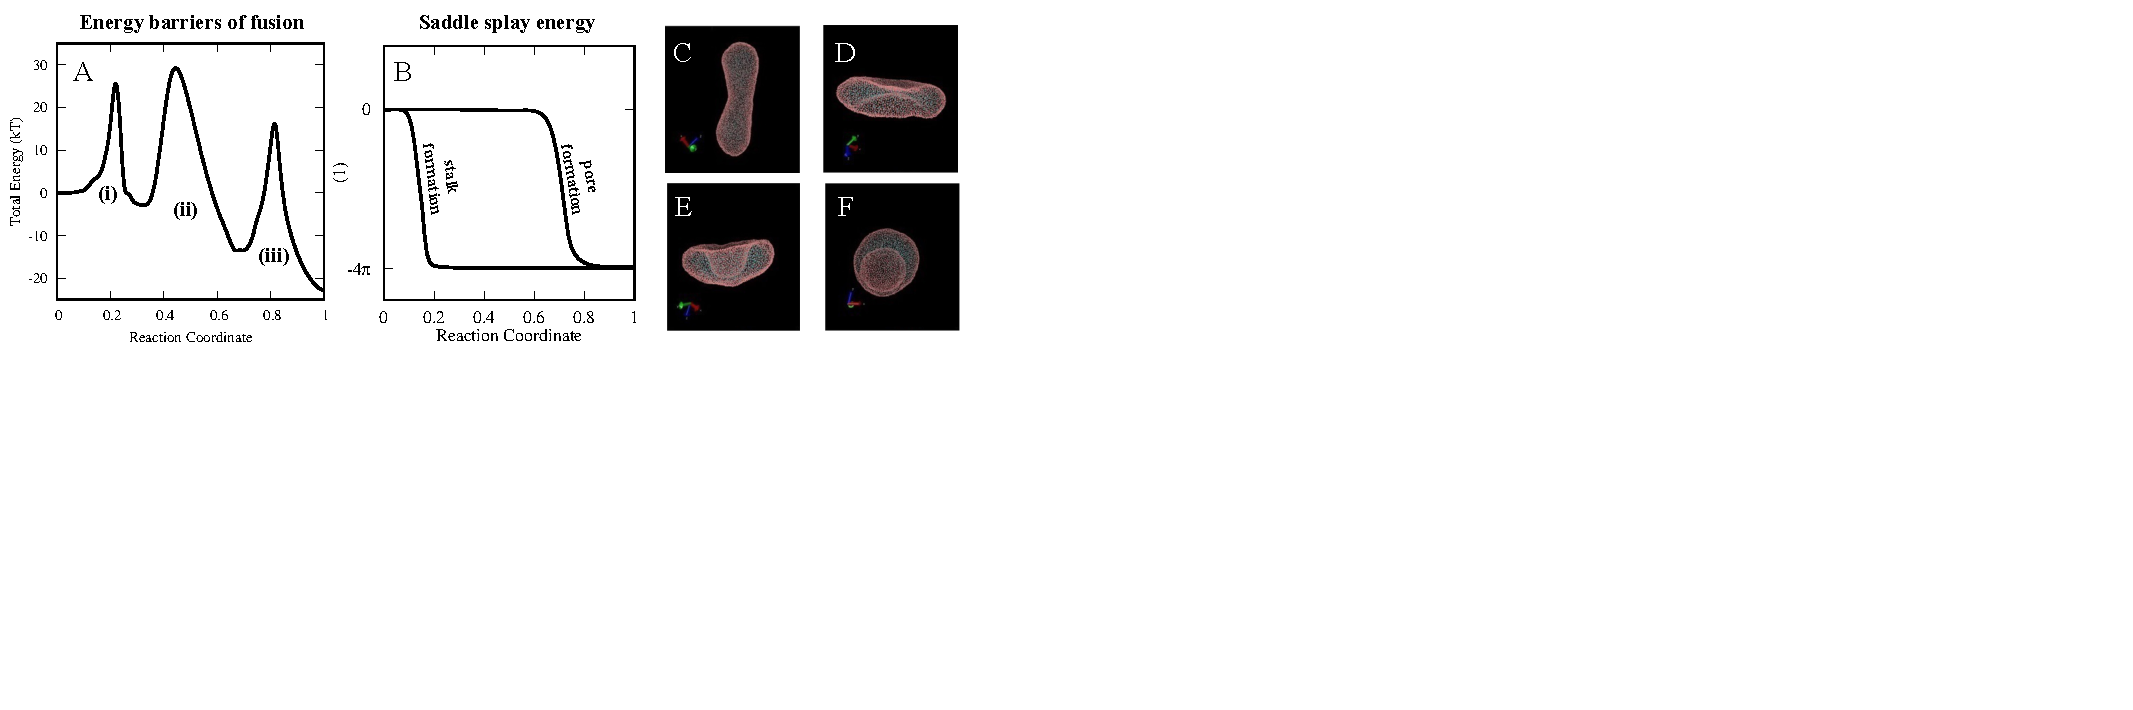
\includegraphics[width=0.5\textwidth]{figures/SA1_fig3.pdf}}
%\caption{{\footnotesize (A) Energy barriers for stalk formation (i), hemifusion
%diaphragm expansion (ii) and pore formation (iii). 
%(B) Saddle-splay energy for each change in \emph{monolayer} topology
%calculated in \cite{RyKlYaCo16}. (C)--(F): Shape transition of vesicle at different values of volume to area ratio from coarse-grained simulations of lipid bilayer membranes \cite{Fu16}.}}
%\label{fig:barriers}
%\end{wrapfigure}

%\begin{center}
%Anticipated model simulations
%\end{center}
\subsubsection{Anticipated model simulations}
To characterize material properties, we compare the energies and forces generated by
a collection of amphiphilic particles against the energies and forces of a continuum bilayer.
The comparison enables us to understand how the model parameters map onto elastic parameters. 

In the preliminary work, bilayer shapes minimized energy with respect to an external force. Energy minimality is somewhat unrealistic because
biological membranes are constantly in motion. Tracking the evolution of a bilayer is a more robust procedure that does not require minimality.
Here we start with a particle bilayer in a non-equilibrium shape, and then evolve the particle bilayer according to steepest gradient descent with respect to the
HARP functional. Gradient descent stabilizes the evolving bilayer shape and gives a monotonically decreasing energy. This gives a relatively large
data set of energy $E$ versus particle configuration. At the same time, we reconstruct an evolving monolayer dividing surface $\Sigma$ and director field $n$ by
interpolating the particle centers and orientations. Using \eqref{ansatz3}, we calculate a continuum energy $H$ from the interpolated
bilayer shape. Setting $\Delta E = E - E_0$ and $\Delta H = H - H_0$ normalizes the energies to their respective equilibrium values $E_0$ and $H_0$.
In certain instances, the bilayer evolution involves only one of the four fundamental deformations.
When this occurs, the elastic moduli appear as the slope of the linear regression between $\Delta H$ and $\Delta E$. 

Bending is the energetically most consequential deformations,
and so we revisit estimating the bending modulus parameter. 
In the case of the bending deformation, we deform the midplane of a planar bilayer into the shape of a circular arc.
This arc stores bending energy in the form of splay $\Div{n}$, while twist, saddle-splay and tilt deformations are zero.
The splay in the two leaflets approximately cancel when added, making the contribution of spontaneous curvature negligible.
Since $\Div{n} = -\kappa$ in this setup, we can compute the curvature squared curvature energy 
$H = \int_C \kappa^2$ of the cross-section $C$, a simple closed curve. Figure \ref{} shows the approximately linear
relationship between $\Delta E$ and $\Delta H$ with $\KB$ as the slope.

The twist deformation is a fully three-dimensional deformation. 
(Specific Aim 3 address outstanding implementation issues like three-dimensional boundary integral solvers.) 
The twist deformation is closely related to the assumption of lateral fluidity in membranes and so researchers 
have sometimes assumed $\KT = 0$ \cite{Hamm2000, TerziDeserno17, C9SM02079A, PhysRevE.102.042406}, 
while molecular dynamics investigations find a twist modulus in the range of 1 to 2 
\kBT \cite{LeVeWa14}.
To measure the elastic response,  we initially twist the bilayer along an $x_1$-coordinate axis.
In this configuration, the directors behave at leading order as $n = (0, mx_1, \sqrt{1 - m^2x_1^2})$,
yielding a surface gradient $\nabla n = \begin{pmatrix}0 & 0\\ m & 0\end{pmatrix}$. 
Here $\Div n = \mathrm{tr}(\nabla n) = 0$, $\det(\nabla n) = 0$ and $\Curl d = (\nabla u)_{12} - (\nabla u)_{21} = m$,
so that the continuum elastic energy equals $\tfrac{1}{2}\KT m^2 A + O(1)$ for a membrane area $A \gg 1$. (Our particle collections
conserve membrane area, unless they lie in a strong background flow.) 
This enables us to plot the HARP energy values derived from steepest gradient descent as a function of $m$, and finally
yields a value for $\KA$. 

We will also determine the effective saddle splay modulus $\KG$. 
Theoretical analysis of lipid phase transitions predict a negative saddle-splay modulus around $-8$ \kBT\;
\cite{SIEGEL2004366,SIEGEL20085200}. Researchers point out, however, that this theoretical value requires a larger energy 
barrier for monolayer fusion than is found by experiment \cite{FrRoPi17,Tran7106,TerziDeserno17}. 
The field requires further theoretical work like the what we are proposing to more precisely account for saddle splay.
  
The gradient descent technique is ineffective for measuring $\KG$ because
the saddle splay energy is largely invariant under shape changes.
In the simplified Canham-Helfrich formulation, saddle splay energy is an indicator of topological transitions, thanks to the  Gauss-Bonnet theorem
\cite{TerziDeserno17}.
PI-Ryham showed that saddle splay acts as a topological indicator even in the presence of nonzero tilt \cite{RyKlYaCo16}. 

To evaluate $\KG$, we will combine the string method from PI-Ryham's work on fusion \cite{RyKlYaCo16} with
the present particle simulations. The string method is a numerical scheme that finds
least energy pathways separating energy basins \cite{doi:10.1063/1.2720838}.
Using the string method, we will evaluate the transition energies between the intact pancake shape,
and one with a pore. Pore formation in a single bilayer decreases the integral of saddle splay from $4\pi$
to $0$. We can, in principle, detect this drop in energy because we have already accounted for the other deformations. 

We will also analyze $\KG$ using a helical geometry. In a helicoid with inclination $m$, the director
gradient is $\nabla n = \begin{pmatrix} 0 & m(m^2+x_1^2)^{-1} \\ m(m^2+x_1^2)^{-1} & 0\end{pmatrix}$ where $x_1$ is the distance to the central
axis. We observe that saddle splay, twist and tilt are zeros, and $\det \nabla n = m^2(m^2+x_1^2)^{-2}$.
In the simulations, the particles forming the helicoid will be confined to two, concentric cylinders. The
continuum energy $\tfrac{1}{2}\KG h(m x_1(m^2+x_1^2)^{-1} + \tan^{-1}(x_1/m)) |_{r_1}^{r_2}$ where $h$, $r_1$ and $r_2$
are the cylinder heights, inner cylinder radius, and outer cylinder radius, respectively. 

The form of the elastic energy density \eqref{ansatz3} is the same as
the Oseen-Frank energy density for nematic liquid crystals \cite{ANDRIENKO2018520,Tran7106,Helfrich73}.   In fact,  
a lipid monolayer acts as one layer in a smectic  phase \cite{REYESMATEO1995978,Rangamani20140463,PhysRevLett.113.248102}. 
The constants $\KB$, $\KT$  and $\KG$ play the same role as the Frank constants $K_1$, $K_2$ and $K_{24}$
liquid crystal theory. However, the ``bend'' distortion from nematics  
is not present in monolayers since the directors have no dependence in the normal direction.
There is also no ``spontaneous twist'' in monolayers due to invariance under mirror reflection. 

 It may come as a surprise then that the field of membrane continuum mechanics still lacks consensus as to
  whether \eqref{ansatz3} contains a complete list of consistent deformations.
  The PI Ryham showed, for example, that the tilt vector $T = n/n\cdot N - N$ leads to unphysical cusps when constraining membrane thickness
 \cite{RyKlYaCo16}.
  Recently, \cite{TerziDeserno17} derived a tilt curvature term that was neglected from the HK analysis \cite{Hamm2000}.
  Later, \cite{C9SM02079A} 
  and \cite{PhysRevE.102.042406} independently identified an inconsistency \cite{TerziDeserno17} arising
  from a transversal tilt invariance assumption. 

  We suspect the reason why, after twenty years, the field has yet to reach a consensus 
  has to do with the Taylor expansions used to derive the elastic energy density. 
  Past researchers expressed the strain tensor in
  terms of the coordinate frame $\{e_1, e_2, N\}$ with surface tangent vectors $e_i$ and surface normal $N$.  
  In this frame, there is a coupling between the gradients of all three terms $x_0,$ $\zeta$ and $n$ of the deformation \eqref{LMdeformation}.
  The recent paper \cite{PhysRevE.102.042406} contains an energy density with more than ten elastic parameters, for example.
  Subtle differential geometric arguments are needed to evaluate the terms in the Taylor expansion.

  We will revisit the HK analysis to see if any inconsitencies can be resolved.
  As a main analytical innovation, we have found that expanding the strain tensor in
  terms of the coordinate frame $\{e'_1, e'_2, n\}$ with $e'_i$ perpendicular to $n$
  greatly simplifies the expansion because it decouples the gradient terms. As an illustration, the prominent works
  \cite{TerziDeserno17, PhysRevE.102.042406, Hamm2000, C9SM02079A} utilize an
  incompressility condition for the lipid elongation function $\zeta$ from \eqref{LMdeformation} that is only approximately true. 
  However, when expressed in the $\{e'_1, e'_2, n\}$ coordinate frame, the incompressility condition is exact
  and is given by a Steiner-type polynomial in terms of $\Div n$ and $\det \nabla n$ \cite{Fe59}.
  Aside from the special case of zero tilt, \cite{Hamm2000} and coworkers seem to have been unaware of this result.

Our investigations will leave open the possibility that the free energy of monolayers and bilayers is non-local. 
We have shown that hydrophic attraction is a non-additive force, meaning the force of attraction between two
particles is dependent on the position a third or more particles. Conceptually, this would arise in continuum theory if two monolayer surfaces
had a different elastic energy density despite having locally identical curvatures and directors.
The boundary integral formulation described in Specific Aim 3 easily accomodates additional linear PDE and
we will extend our study to include charge lipids and weak electrolytes \cite{C9SM00772E}.

